\begin{myChapterIntro}{本章内容涵盖}
\begin{itemize}
\item 从 LLM 回复中可靠地提取最终答案
\item 借助符号数学求解器，把 LLM 的输出与参考答案对比，从而验证答案是否正确
\item 运行完整的评估流水线：加载预训练模型、生成输出，并对照数据集为其打分
\end{itemize}
\end{myChapterIntro}

评估让我们能够区分那些只是听起来有说服力的 LLM，和真正能正确解决问题的 LLM。LLM 评估技术涵盖的方法十分广泛，从衡量任务准确率，到确保 LLM 符合特定的安全标准。本章中，“评估”指的是在大量样本上定量地测试模型，并对照参考答案为其输出打分。

更具体地说，我们将重点实现一种基于\emph{验证}的方法，它借助一个类似计算器的实现，把模型的答案与参考答案进行对比，从而检查 LLM 能否准确地求解数学问题。

这个验证器格外有用，因为它不仅能评估数学任务上的表现，还引入了\emph{可验证奖励}的原理——而这正是我们将在第 6 章实现、用于推理模型的强化学习方法的基础。

\section{构建数学验证器}

实践中，评估训练好的 LLM 有四种常见方式：\emph{选择题}、\emph{验证器}、\emph{排行榜}和 \emph{LLM 评审}。这些方法广泛用于研究论文、技术报告、营销材料和模型卡（用于说明模型如何训练、如何评估以及预期用途的文档）中，而且评估结果往往来自不止一种方式。

如图 3.1 所示，这些评估方法可以归为两大类：\emph{基于基准测试的评估}和\emph{基于判断的评估}。前者通常更偏定量，后者则更依赖定性判断。这四种评估方法在不同场景下各有其用，但对推理模型来说，验证器尤为重要。

\myGraphic{0.92}{images/CH03_F01_Raschka2.png}{图 3.1 本书涵盖主题的模型图。本章讨论评估方法（第 2 阶段），并特别聚焦于实现验证器，我们将在第 6 章把它复用为可验证奖励的基础。}

数学问题是一个天然的示例：根据问题复杂程度的不同，它们能从逐步推理中获益，而评估又很直接，因为最终答案可以与正确答案对照检查。在这种情况下，验证器提供了一种简单而可靠的方式，用来衡量模型的推理步骤是否导向正确结果。

本章中，我们将重点讨论把验证器作为一种基于基准测试的方法，用来衡量数学问题中答案的正确性。如图 3.2 所示，验证器会将提取出的答案与参考答案进行对比，且往往会借助代码解释器或计算器程序等外部工具。

\myGraphic{0.92}{images/CH03_F02_Raschka2.png}{图 3.2 在自由形式问答中用基于验证的方法评估 LLM。模型生成一段自由形式的答案（可能包含多个步骤）以及一个最终答案框，后者会被提取出来，并与数据集中的正确答案进行比较。}

\begin{myWarning}{注意}
 附录 F 介绍了其他评估方法，比如选择题基准测试、基于偏好的排行榜，以及 LLM 作为评审的方法。\end{myWarning}

虽然我们眼下的重点是评估，但验证器在本书后面还会再次出现。它不仅是衡量表现的手段，也是强化学习方法训练推理模型时所用的反馈信号，这一点我们将在第 6 章探讨。

其缺点在于，验证器方法只能应用于那些能够被轻松（最好还能确定性地）验证的领域，比如数学和代码。此外，这种做法会带来额外的复杂性和依赖，还可能把一部分评估负担从模型本身转移到外部工具上。

由于数学题可以通过程序无限地生成各种变体，而且它们能从逐步推理中获益，因此这项任务已成为评估和开发推理模型的基石。本章中，我们将按照图 3.3 所示的八个步骤，逐步构建一个数学验证器。

\myGraphic{0.92}{images/CH03_F03_Raschka2.png}{图 3.3 构建并应用数学验证器的分步工作流。从一个预训练 LLM 出发，我们生成答案、提取并规范化答案，然后将其与标准答案对比。验证后的答案随后被打分，并在整个数据集（MATH-500）上重复这一过程，以评估模型的整体表现。}

下一节将介绍图 3.3 中的第 1 步和第 2 步：加载一个预训练 LLM，并把它配置好来生成答案。

\section{加载预训练模型以生成文本}

本节中，我们开始实现验证器，先加载上一章介绍的预训练 LLM，并把它配置好以生成答案。这将为图 3.3 中后续步骤打下基础，届时我们会提取、规范化并验证这些答案。它还会为后面几章搭好一条可复用的模型加载路径，因为那时我们需要对比不同的推理方法，并需要一种一致的方式来衡量它们是否真的提升了模型。

我们将使用第 2 章用过的同一个预训练基础模型。为了方便并便于后续章节复用，我们会把模型加载逻辑封装进一个 \texttt{load\_model\_and\_tokenizer} 函数调用，如下面的代码清单所示。

\begin{codeboxt}{代码清单 3.1 加载预训练模型}
from pathlib import Path
import torch

from reasoning_from_scratch.ch02 import (
    get_device
)
from reasoning_from_scratch.qwen3 import (
    download_qwen3_small,
    Qwen3Tokenizer,
    Qwen3Model,
    QWEN_CONFIG_06_B
)

def load_model_and_tokenizer(
    which_model, device, use_compile, local_dir="qwen3"
):
    if which_model == "base":

        download_qwen3_small(
            kind="base", tokenizer_only=False, out_dir=local_dir
        )

        tokenizer_path = Path(local_dir) / "tokenizer-base.json"
        model_path = Path(local_dir) / "qwen3-0.6B-base.pth"
        tokenizer = Qwen3Tokenizer(tokenizer_file_path=tokenizer_path)

    elif which_model == "reasoning":

        download_qwen3_small(
            kind="reasoning", tokenizer_only=False, out_dir=local_dir
        )

        tokenizer_path = Path(local_dir) / "tokenizer-reasoning.json"
        model_path = Path(local_dir) / "qwen3-0.6B-reasoning.pth"
        tokenizer = Qwen3Tokenizer(
            tokenizer_file_path=tokenizer_path,
            apply_chat_template=True,
            add_generation_prompt=True,
            add_thinking=True,
        )

    else:
        raise ValueError(f"Invalid choice: which_model={which_model}")

    model = Qwen3Model(QWEN_CONFIG_06_B)
    model.load_state_dict(torch.load(model_path))

    model.to(device)

    if use_compile:  #1
        torch._dynamo.config.allow_unspec_int_on_nn_module = True
        model = torch.compile(model)

    return model, tokenizer

WHICH_MODEL = "base"   #2
device = get_device()
# device = torch.device("cpu")  #3

model, tokenizer = load_model_and_tokenizer(
    which_model=WHICH_MODEL,
    device=device,
    use_compile=False
)
\end{codeboxt}
{\noindent\small\textit{\#1 可选：设为 true 以启用模型编译。 \newline \#2 默认使用基础模型，与第 2 章类似 \newline \#3 如果你的设备存在兼容性问题，请取消注释这一行。}\par}

默认情况下，代码清单 3.1 会加载基础模型，与第 2 章一样。

一个可选的变体是官方的 Qwen3 推理模型，Qwen3 团队用专门面向推理的方法在基础模型之上训练出了它。它并不是我们将在本书后面构建的自定义推理模型。这里我们只是把它当作一个参照点。你可以在代码清单 3.1 中设置 \texttt{WHICH\_MODEL = }\texttt{"}\texttt{reasoning}\texttt{"} 来加载它，以便之后将其评估结果与基础模型的评估结果进行比较。

现在模型已经加载完成，我们可以用第 2 章的文本生成函数来生成文本，如下面的代码清单所示。

\begin{codeboxt}{代码清单 3.2 生成模型输出}
from reasoning_from_scratch.ch02 import (
    generate_text_basic_stream_cache
)

prompt = (  #1
    r"If $a+b=3$ and $ab=\tfrac{13}{6}$, "
    r"what is the value of $a^2+b^2$?"
)

input_token_ids_tensor = torch.tensor(  #2
    tokenizer.encode(prompt),
    device=device
).unsqueeze(0)  #3

all_token_ids = []

for token in generate_text_basic_stream_cache(  #4
    model=model,
    token_ids=input_token_ids_tensor,
    max_new_tokens=2048,
    eos_token_id=tokenizer.eos_token_id
):
    token_id = token.squeeze(0)  #5
    decoded_id = tokenizer.decode(token_id.tolist())
    print(  #6
        decoded_id,
        end="",
        flush=True
    )
    all_token_ids.append(token_id)

all_tokens = tokenizer.decode(all_token_ids)  #7
\end{codeboxt}
{\noindent\small\textit{\#1 把数学题定义为一个字符串提示。 \newline \#2 把提示转换成模型能够处理的词元 ID。 \newline \#3 增加批量维度 \newline \#4 让模型一次生成一个输出词元。 \newline \#5 移除批量维度 \newline \#6 在词元生成时打印它 \newline \#7 把完整生成序列解码为文本。}\par}

在这个代码清单中，我们先把一道简单的数学题编码成模型能够处理的词元 ID。随后模型以流式方式逐个生成词元。我们会在词元出现时立刻把它打印出来，这样就能在生成过程中读取输出。与此同时，我们把这些生成的词元收集到一个列表里，以便之后把它们解码成最终的答案字符串。这种既流式输出又收集词元的模式很实用，因为它让我们能实时监控生成过程，同时仍然保存完整的答案文本（存于 \texttt{all\_tokens}），供后续处理。

代码清单 3.2 中的代码生成的回复如下：

\begin{codebox}
To find the value of \( a^2 + b^2 \) given that \( a + b = 3 \)
and \( ab = \frac{13}{6} \), we can use the following algebraic identity:

\[
a^2 + b^2 = (a + b)^2 - 2ab
\]

**Step 1:** Substitute the given values into the equation.

\[
a^2 + b^2 = (3)^2 - 2 \left( \frac{13}{6} \right)
\]

[...]  #1

**Final Answer:**

\[
\boxed{\dfrac{14}{3}}
\]
\end{codebox}
{\noindent\small\textit{\#1 为简洁起见已作删减}\par}

从这个回复可以看出，尽管我们用的是基础模型，它却给出了类似推理模型的解释。这很可能是因为 Qwen3 团队在预训练时加入了思维链（chain-of-thought, CoT）数据，正如他们的技术报告所述。不过，即便模型表现出一些类似推理模型的行为，加入额外的推理方法仍能进一步提升这些能力。（请注意，生成的回复可能因代码运行在 CPU、CUDA 还是 MPS 设备上而有所不同。）

如果你不熟悉数学中常用的 LaTeX 语法，前面的回复可能不太好读懂。这种情况下，你可以用 IPython 的 \texttt{Latex} 类来渲染它：

\begin{codebox}
from IPython.display import Latex, display
display(Latex(all_tokens))
\end{codebox}

在代码笔记本中运行上述代码的结果如图 3.4 所示。

\myGraphic{0.92}{images/CH03_F04_Raschka2.png}{图 3.4 渲染后的回复，包含逐步计算过程和最终的答案框}

图 3.4 中显示的最终答案确实是这道题的正确答案。

\section{实现一个便于文本生成的封装}

我们已经加载好预训练 LLM 并搭好了文本生成功能（如图 3.5 所示）。现在，为了方便后续章节使用，我们会为文本生成函数创建一个封装（见代码清单 3.3），这样每次只需传入模型、分词器和提示，再加一些额外设置，而不必重复分词和输入准备步骤。

\myGraphic{0.92}{images/CH03_F05_Raschka2.png}{图 3.5 本节中，我们把验证器工作流的第 1 步和第 2 步封装成一个可复用的文本生成辅助函数。封装会处理提示构造和流式生成，并返回模型原始的 LaTeX 输出，这样就不必每次都重复分词和输入准备。}

\begin{codeboxt}{代码清单 3.3 流式文本生成的封装}
def generate_text_stream_concat(
    model, tokenizer, prompt, device, max_new_tokens,
    verbose=False,
):
    input_ids = torch.tensor(                    #1
        tokenizer.encode(prompt), device=device
        ).unsqueeze(0)

    generated_ids = []
    for token in generate_text_basic_stream_cache(  #2
        model=model,
        token_ids=input_ids,
        max_new_tokens=max_new_tokens,
        eos_token_id=tokenizer.eos_token_id,
    ):
        next_token_id = token.squeeze(0)
        generated_ids.append(next_token_id.item())

        if verbose: #3
            print(
                tokenizer.decode(next_token_id.tolist()),
                end="",
                flush=True
            )

    return tokenizer.decode(generated_ids)  #4
\end{codeboxt}
{\noindent\small\textit{\#1 把提示文本编码为词元 ID 并放到设备上。 \newline \#2 使用带缓存的生成方式逐个流式输出词元。 \newline \#3 可选：在词元生成时打印它们。 \newline \#4 把所有生成的 ID 解码为最终的文本字符串。}\par}

这个封装函数负责文本生成的全流程：对输入提示进行分词，从模型流式获取新词元，然后把结果解码成最终字符串。

如前所述，可选的 verbose 标志让我们能实时看到正在生成的词元。这个函数的用法如下：

\begin{codebox}
generated_text = generate_text_stream_concat(
    model, tokenizer, prompt, device,
    max_new_tokens=2048,
    verbose=True  #1
)
\end{codebox}
{\noindent\small\textit{\#1 使用 False 会关闭逐个词元的实时打印。}\par}

这段代码打印出的回复与你在 3.2 节看到的完全一致：

\begin{codebox}
[...]  #1

**Final Answer:**

\[
\boxed{\dfrac{14}{3}}
\]
\end{codebox}
{\noindent\small\textit{\#1 为简洁起见已作删减}\par}

\section{提取最终答案框}

现在模型已经加载就绪，我们可以进入有趣的部分了：评估模型。

值得回想一下，本书采用从零实现的思路，这自然意味着要涉及一些细致、有时甚至繁琐的步骤。这是有意为之。我们希望亲手构建评估流水线，从而更好地理解它的运作方式，而不是只调用现成的封装函数和构件。

上一节中，你看到模型把最终答案放在一个答案框里返回（在原始文本中写作 \texttt{r}\texttt{"}\texttt{\textbackslash{}boxed\{\textbackslash dfrac\{14\}\{3\}\}}\texttt{"}）。我们并没有强制要求这种格式；模型之所以这样输出，很可能是因为答案框是数学基准测试和训练数据中的常见惯例。这种行为未必能证明模型对我们将要运行的评估任务过拟合，但它反映出预训练模型在网上会经常遇到各种题目格式，并学会复现这些风格上的惯例。一般来讲，可以合理地认为，模型训练时互联网上可获取的任何信息都曾是训练数据的一部分。

虽然这里并不需要，但之后我们在 MATH-500 数据集上评估模型时，会加入一个特定的提示，指示模型以这种答案框的形式返回答案。（MATH-500 是经过整理的 500 道题的集合，被广泛用作推理模型的基准数据集。）这一步很直接，而且每当我们需要把模型回复转换成能够大规模自动打分的形式时，都会用到它。这种常见的惯例让不同模型之间的评估更加一致，也简化了数据提取。

下面我们来编写代码，完成对答案框内容的提取。本节实现图 3.6 中的第 3 步。（下一节将实现第 4 步所需的规范化方法。）

\myGraphic{0.92}{images/CH03_F06_Raschka2.png}{图 3.6 从 LLM 输出中提取答案框结果的示意图}

由于受硬件影响，你的模型可能生成与我这里略有不同的回复，所以下面的代码使用一个硬编码的占位答案，而不是让模型实际生成回复（不过我们就当这个答案是模型生成的）。在后面几节中，我们会回到模型，让它为 MATH-500 数据集中的任务生成答案：

\begin{codebox}
model_answer = (
r"""... some explanation...
**Final Answer:**

\[                     #1
\boxed{\dfrac{14}{3}}   #1
\]                      #1
""")
\end{codebox}
{\noindent\small\textit{\#1 我们想要提取的答案框}\par}

\begin{myWarning}{注意}
 我们使用的是原始字符串（\texttt{r}\texttt{"""}\texttt{...}\texttt{"""}，而不是普通字符串 \texttt{"""}\texttt{...}\texttt{"""}）。原始字符串更便于处理反斜杠（\texttt{\textbackslash}）字符，否则反斜杠会被当作转义序列，每个反斜杠都得写成两个。\end{myWarning}

接下来，我们定义一个函数，从 \texttt{model\_answer} 中提取答案框。

\begin{codeboxt}{代码清单 3.4 提取答案框}
def get_last_boxed(text):
    boxed_start_idx = text.rfind(r"\boxed")  #1
    if boxed_start_idx == -1:
        return None

    current_idx = boxed_start_idx + len(r"\boxed")  #2

    while current_idx < len(text) and text[current_idx].isspace():#3
        current_idx += 1

    if current_idx >= len(text) or text[current_idx] != "{":#4
        return None

    current_idx += 1
    brace_depth = 1
    content_start_idx = current_idx

    while current_idx < len(text) and brace_depth > 0:#5
        char = text[current_idx]
        if char == "{":
            brace_depth += 1
        elif char == "}":
            brace_depth -= 1
        current_idx += 1

    if brace_depth != 0:  #6
        return None

    return text[content_start_idx:current_idx-1]  #7
\end{codeboxt}
{\noindent\small\textit{\#1 找到最后一次出现的“\textbackslash{}boxed”。 \newline \#2 获取“\textbackslash{}boxed”之后的位置。 \newline \#3 跳过“\textbackslash{}boxed”之后的空白字符。 \newline \#4 期望遇到一个左花括号“\{”。 \newline \#5 按嵌套层级解析花括号。 \newline \#6 处理花括号不配对的情况。 \newline \#7 提取最外层花括号内的内容。}\par}

代码清单 3.4 中的辅助工具函数 \texttt{get\_last\_boxed} 会从模型输出中提取最后一个 \texttt{\textbackslash{}boxed\{...\}} 表达式的内容。更具体地说，它会扫描出最后一个 \texttt{\textbackslash{}boxed}，跳过空白字符，检查花括号，并处理嵌套，从而捕获到我们想要的答案字符串。

虽然这个解析器看起来有些繁琐，但等到我们在 MATH-500 这类数据集上跑评估时，它的价值就会显现出来——因为提取出正确的最终答案，是衡量模型推理能力的第一步。

现在，我们在模型答案上测试这个函数：

\begin{codebox}
extracted_answer = get_last_boxed(model_answer)
print(extracted_answer)
\end{codebox}

这个函数调用的输出是 \texttt{"}\texttt{\textbackslash dfrac\{14\}\{3\}}\texttt{"}，正是我们想要提取的答案框内容。

\begin{mySidebar}{渲染数学公式}

我们可以通过前面介绍的 \texttt{Latex} 类来渲染数学公式。如果是没有配套答案文本的独立数学公式，也可以改用更简单的 \texttt{Math} 类：

\begin{codebox}
from IPython.display import Math
display(Math(r"\dfrac{14}{3}"))
\end{codebox}

这会把该分数渲染为

\begin{center}
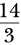
\includegraphics[width=0.025\linewidth, valign=c]{images/26.jpg}
\end{center}

\end{mySidebar}

前面的 \texttt{get\_last\_boxed} 函数正确地提取出了文本，但我们可以用 \texttt{extract\_final\_candidate} 函数（见下面的代码清单）让答案提取更稳健一些，它会处理最终答案框缺失或不完整的情况。

\begin{codeboxt}{代码清单 3.5 提取最终答案候选}
import re

RE_NUMBER = re.compile(  #1
    r"-?(?:\d+/\d+|\d+(?:\.\d+)?(?:[eE][+-]?\d+)?)"
)

def extract_final_candidate(text, fallback="number_then_full"):

    result = ""  #2

    if text:  #3
        boxed = get_last_boxed(text.strip())
        if boxed:
            result = boxed.strip().strip("$ ")

        elif fallback in ("number_then_full", "number_only"):#4
            m = RE_NUMBER.findall(text)
            if m:
                result = m[-1]  #5
            elif fallback == "number_then_full":

                result = text  #6
    return result
\end{codeboxt}
{\noindent\small\textit{\#1 用于从文本中提取数值的正则表达式 \newline \#2 没有任何匹配时的默认返回值 \newline \#3 如果存在答案框表达式，优先使用最后一个。 \newline \#4 如果没有答案框表达式，则尝试回退方案。 \newline \#5 使用最后一个数字。 \newline \#6 否则，如果没有找到数字，就返回完整文本。}\par}

\texttt{extract\_final\_candidate} 函数提供了 \texttt{fallback} 设置，以应对找不到答案框的情况，具体如下：

\begin{itemize}
\item \texttt{"}\texttt{number\_then\_full}\texttt{"}（默认值）：选取最后一个简单数字；否则选取整段文本。
\item \texttt{"}\texttt{number\_only}\texttt{"}：选取最后一个简单数字；否则返回空字符串 \texttt{""}。
\item \texttt{"}\texttt{none}\texttt{"}：只提取答案框中的内容；否则返回空字符串 \texttt{""}。
\end{itemize}

对于回退设置，代码清单 3.5 中的代码使用了\emph{正则表达式}（简称 regex），它借助 Python 的 \texttt{re} 库实现。正则表达式是一种在文本中搜索模式的方式。在我们的例子里，正则模式用于识别数字，包括分数、小数和科学计数法。虽然正则语法看起来令人生畏，但这里不必费心去弄懂它的运作细节。重要的是，它为我们提供了一件可靠的工具：当没有答案框时，从模型输出中提取最后一个数字候选。

我们在模型答案上试一试：

\begin{codebox}
print(extract_final_candidate(model_answer))
\end{codebox}

它正确地返回了 \texttt{"}\texttt{\textbackslash dfrac\{14\}\{3\}}\texttt{"}。

现在我们再看几个额外的例子。首先，另一个带答案框的候选：

\begin{codebox}
print(extract_final_candidate(r"\boxed{ 14/3. }"))
\end{codebox}

它正确地返回了 \texttt{"}\texttt{14/3.}\texttt{"}，去掉了多余的空白字符，但没有去掉标点。这个标点字符会被我们后面实现的相等性检查正确处理。

接下来，我们试一个不带答案框的候选，这应当触发回退设置：

\begin{codebox}
print(extract_final_candidate("abc < > 14/3 abc"))
\end{codebox}

得益于默认的回退设置，它会找到答案中的最后一个数字，并正确地返回 \texttt{"}\texttt{14/3}\texttt{"}。

本节中，我们定义了一些工具函数，用于从 LLM 的回复文本中提取答案。这让我们朝着验证答案是否正确这一总体目标又迈进了一步。下一节中，我们会先把回复规范化成更通用的标准形式，然后再实现检查功能。

\begin{mySidebar}{为什么不直接用 LLM 来提取答案？}

我们当然可以用 LLM 来提取答案框内容本身，但那样会引入不必要的复杂性和潜在错误。假设 LLM 会按特定格式输出答案，那么提取就是一项简单、机械的任务：我们只需定位最后一个答案框表达式，如果它不存在，就回退到某个数字或原始文本。

正则表达式乍看之下可能很复杂，但我们现在已经得到了一个小巧、可复用的工具函数，它运行开销低，能确定、可复现地完成提取，不必依赖于另一个模型输出的波动。

\end{mySidebar}

\section{规范化提取出的答案}

前面我们从模型回复中提取出了答案框 \texttt{"}\texttt{\textbackslash dfrac\{14\}\{3\}}\texttt{"}。同一个值可能有多种写法，比如 \texttt{"}\texttt{\textbackslash frac\{14\}\{3\}}\texttt{"}、\texttt{"}\texttt{14/3}\texttt{"}、\texttt{"}\texttt{\$14/3\$}\texttt{"} 或 \texttt{"}\texttt{(14)/(3)}\texttt{"}。要实现并使用一套稳健的检查体系来判断答案是否正确，我们首先需要一种一致的比较方式。本节中，我们将实现一次规范化（或称标准化）处理（图 3.7 中的第 4 步），用以剥离格式并统一答案。

\myGraphic{0.92}{images/CH03_F07_Raschka2.png}{图 3.7 从 LLM 输出中提取答案框结果，并将其转换为标准朴素形式的示意图。这个规范化后的答案稍后将与正确答案进行验证比对。}

图 3.7 所示的规范化步骤由下面的 \texttt{normalize\_­text} 函数实现。

\begin{codeboxt}{代码清单 3.6 规范化提取出的答案}
LATEX_FIXES = [  #1
    (r"\\left\s*", ""),
    (r"\\right\s*", ""),
    (r"\\,|\\!|\\;|\\:", ""),
    (r"\\cdot", "*"),
    (r"\u00B7|\u00D7", "*"),
    (r"\\\^\\circ", ""),
    (r"\\dfrac", r"\\frac"),
    (r"\\tfrac", r"\\frac"),
    (r"°", ""),
]

RE_SPECIAL = re.compile(r"<\|[^>]+?\|>")  #2
SUPERSCRIPT_MAP = {
    "⁰": "0", "¹": "1", "²": "2", "³": "3", "⁴": "4",  #3
    "⁵": "5", "⁶": "6", "⁷": "7", "⁸": "8", "⁹": "9",     #3
    "⁺": "+", "⁻": "-", "⁽": "(", "⁾": ")",               #3
}

def normalize_text(text):
    if not text:
        return ""
    text = RE_SPECIAL.sub("", text).strip()

    match = re.match(r"^[A-Za-z]\s*[.:]\s*(.+)$", text)#4
    if match: #4
        text = match.group(1) #4
 #4
 #4
    text = re.sub(r"\^\s*\{\s*\\circ\s*\}", "", text)   #4
    text = re.sub(r"\^\s*\\circ", "", text)            #5
    text = text.replace("°", "")                        #5

    match = re.match(r"^\\text\{(?P<x>.+?)\}$", text)  #6
    if match:
        text = match.group("x")

    text = re.sub(r"\\\(|\\\)|\\\[|\\\]", "", text)  #7

    for pat, rep in LATEX_FIXES:  #8
        text = re.sub(pat, rep, text)

    def convert_superscripts(s, base=None):
        converted = "".join(
            SUPERSCRIPT_MAP[ch] if ch in SUPERSCRIPT_MAP else ch
            for ch in s
        )
        if base is None:
            return converted
        return f"{base}**{converted}"

    text = re.sub(
        r"([0-9A-Za-z\)\]\}])([⁰¹²³⁴⁵⁶⁷⁸⁹⁺⁻]+)",
        lambda m: convert_superscripts(m.group(2), base=m.group(1)),
        text,
    )
    text = convert_superscripts(text)

    text = text.replace("\\%", "%").replace("$", "").replace("%", "")#9
    text = re.sub(
        r"\\sqrt\s*\{([^}]*)\}",
        lambda match: f"sqrt({match.group(1)})",
        text,
    )
    text = re.sub(
        r"\\sqrt\s+([^\\\s{}]+)",
        lambda match: f"sqrt({match.group(1)})",
        text,
    )

    text = re.sub(#10
        r"\\frac\s*\{([^{}]+)\}\s*\{([^{}]+)\}",
        lambda match: f"({match.group(1)})/({match.group(2)})",
        text,
    )
    text = re.sub(
        r"\\frac\s+([^\s{}]+)\s+([^\s{}]+)",
        lambda match: f"({match.group(1)})/({match.group(2)})",
        text,
    )

    text = text.replace("^", "**")#11
    text = re.sub(
        r"(?<=\d)\s+(\d+/\d+)",
        lambda match: "+" + match.group(1),
        text,
    )

    text = re.sub(#12
        r"(?<=\d),(?=\d\d\d(\D|$))",
        "",
        text,
    )

    return text.replace("{", "").replace("}", "").strip().lower()
\end{codeboxt}
{\noindent\small\textit{\#1 需要替换的 LaTeX 格式（左：原值，右：新值） \newline \#2 去掉 \textless{}|assistant|\textgreater{} 之类的聊天特殊词元。 \newline \#3 用于把 Unicode 上标转换为纯文本上标的字典映射 \newline \#4 去掉开头的选择题标签（例如“c. 3” → 3）。 3）。 \newline \#5 移除角度符号。 \newline \#6 如果整个字符串都被“\textbackslash text\{...\}”包裹，则把它拆掉。 \newline \#7 去掉行内/独立数学公式的包裹符：\textbackslash ( \textbackslash ) \textbackslash [ \textbackslash ]。 \newline \#8 LaTeX 标准化 \newline \#9 规范化数字和根式表达式。 \newline \#10 把 LaTeX 分数转换为除法形式。 \newline \#11 处理指数和带分数。 \newline \#12 去掉数字中的千位分隔符。}\par}

这个 \texttt{normalize\_text} 函数接收提取出的答案字符串，并把它改写成标准格式，以便我们可靠地与参考答案比较。它首先去掉特殊词元和多余的 LaTeX 冗余成分，比如 \texttt{\textbackslash left}、\texttt{\textbackslash right} 或度数符号；然后拆掉 \texttt{\textbackslash text\{...\}} 这类包裹、移除行内数学标记，并把常见结构改写成计算器风格的形式。例如，它会把 \texttt{\textbackslash sqrt\{a\}} 变成 \texttt{sqrt(a)}，把 \texttt{\textbackslash frac\{a\}\{b\}} 变成 \texttt{(a)/(b)}。最后，它会规范化指数、带分数和千位分隔符，并清理花括号和大小写。简而言之，这个函数把格式各异的 LaTeX 输出转换成干净、标准化的字符串表示。

我们在模型答案上试一试 \texttt{normalize\_text} 函数：

\begin{codebox}
print(normalize_text(extract_final_candidate(model_answer)))
\end{codebox}

它不会以 LaTeX 格式（\texttt{r}\texttt{"}\texttt{\textbackslash dfrac\{14\}\{3\}}\texttt{"}）输出答案，而是返回一种标准化的、不含 LaTeX 的形式：

\begin{codebox}
"(14)/(3)"
\end{codebox}

接下来，我们试一个格式不同的答案：

\begin{codebox}
print(normalize_text(r"\text{\[\frac{14}{3}\]}"))
\end{codebox}

如预期那样，它同样返回 \texttt{"}\texttt{(14)/(3)}\texttt{"}。

现在我们已经有了一套稳健的方法，可以从 LLM 的回复中提取答案文本。下一节中，我们将实现一个函数，把 LLM 的答案与正确的参考答案进行比较。

\section{验证数学等价性}

到目前为止，我们已经实现了让 LLM 生成答案、提取相关片段并对其进行规范化的各个步骤。如图 3.8 所示，下一步是把提取出的答案与正确的参考答案进行对比来加以验证，在技术语境中，参考答案被称为\emph{标准答案}（ground truth）。我们将在第 6 章再次使用这种验证器来构造可验证的奖励信号，并在后面几章用它来检查训练中的改动是否让模型变得更好。

\myGraphic{0.92}{images/CH03_F08_Raschka2.png}{图 3.8 将 LLM 生成的答案与正确的参考答案（标准答案）进行核对的示意图。LLM 的最终答案框内容被提取、规范化，并与数据集中给出的正确答案进行比较。如果二者一致，该回复就被判定为正确。}

请注意，要实现图 3.8 所示的相等性检查，仅用 Python 的 \texttt{==} 运算符做直接比较是不够的，因为像 \texttt{"}\texttt{14/3}\texttt{"} 和 \texttt{"}\texttt{(14)/(3)}\texttt{"} 这样的表达式不会被判定为相同，而 \texttt{"}\texttt{(28)/(6)}\texttt{"} 与 \texttt{"}\texttt{(14)/(3)}\texttt{"} 这类等价但未经规范化的分数同样会被视为不相等。

在相等性检查中，我们会加入一个中间步骤：用符号数学引擎解析提取并规范化后的答案。为此，我们将使用开源的 SymPy 数学库（\href{https://sympy.org}{https://sympy.org}），它经过二十多年的开发和检验，已成为 Python 科学计算中的常用组件。解析函数在代码清单 3.7 中实现。

\begin{myWarning}{注意}
 如果你还没有安装第 2 章中的依赖，可以用 \texttt{uv} \texttt{pip} \texttt{install} \texttt{sympy}（或 \texttt{uv} \texttt{add} \texttt{sympy}）手动安装 SymPy。\end{myWarning}

\begin{codeboxt}{代码清单 3.7 使用 SymPy 解析器进行数学相等性检查}
from sympy.parsing import sympy_parser as spp
from sympy.core.sympify import SympifyError
from sympy.polys.polyerrors import PolynomialError
from tokenize import TokenError

def sympy_parser(expr):
    if expr is None or len(expr) > 2000: #1
        return None

    try:
        return spp.parse_expr(
            expr,
            transformations=(
                *spp.standard_transformations,  #2

                spp.implicit_multiplication_application,#3
            ),

            evaluate=True,  #4
        )
    except (SympifyError, SyntaxError, TypeError, AttributeError,
            IndexError, TokenError, ValueError, PolynomialError):
        return None
\end{codeboxt}
{\noindent\small\textit{\#1 避免在遇到很长的无效回复时崩溃 \newline \#2 标准变换，例如处理括号 \newline \#3 允许省略乘号（例如 2y → 2*y）。 2*y）。 \newline \#4 在解析时求值，使简单常量得以化简（例如 2+3 → 5）。 5）。}\par}

这个 \texttt{sympy\_parser} 函数接收一个输入表达式（比如我们从 LLM 回复中提取并规范化后的答案），并把它转换成 SymPy 对象，从而能够可靠地比较数学等价性。为此，它应用 SymPy 的标准解析规则，支持隐式乘法（例如写 2\emph{y} 而不是 2 * \emph{y}），并对基本算术进行化简（因此 2 + 3 会变成 5）。

\begin{myWarning}{注意}
 \texttt{sympy\_parser} 处理了看起来数量过多的错误情形，但这些全都是我在用 500 道 MATH-500 题评估模型时实际遇到过的错误。模型并不总能生成格式完美的输出。\end{myWarning}

我们来看看 \texttt{sympy\_parser} 的实际效果，把它用在一个规范化后的答案候选上：

\begin{codebox}
print(sympy_parser(normalize_text(
    extract_final_candidate(model_answer)
)))
\end{codebox}

它返回分数 \texttt{14/3}。接下来，我们试一个未规范化的分数：

\begin{codebox}
print(sympy_parser("28/6"))
\end{codebox}

同样地，它返回 \texttt{14/3}。

有了 \texttt{sympy\_parser}，我们现在就可以实现相等性检查函数了。

\begin{codeboxt}{代码清单 3.8 使用 SymPy 的相等性检查函数}
from sympy import simplify

def equality_check(expr_gtruth, expr_pred):
    if expr_gtruth == expr_pred:  #1
        return True

    gtruth, pred = sympy_parser(expr_gtruth), sympy_parser(expr_pred)#2

    if gtruth is not None and pred is not None:  #3
        try:
            return simplify(gtruth - pred) == 0  #4
        except (SympifyError, TypeError):
            pass

    return False
\end{codeboxt}
{\noindent\small\textit{\#1 首先检查两个表达式是否为完全相同的字符串。 \newline \#2 把两个表达式都解析为 SymPy 对象（解析失败则返回 None）。 \newline \#3 如果两个表达式都解析成功，则尝试符号比较。 \newline \#4 如果差为 0，则二者等价。}\par}

上面代码清单中的 \texttt{equality\_check} 函数用于判断模型的答案是否与标准答案一致。它首先查找完全相同的字符串，这是最简单的情形。如果字符串不同，它就（借助我们在代码清单 3.7 中实现的 \texttt{sympy\_parser} 函数）把两个表达式解析为 SymPy 对象，并检查二者之差是否化简为零。这样我们就能识别出表面上看起来不同（例如 14/3 和 28/6）但在数学上相同的答案。

我们在一个例子上试试代码清单 3.8 中的相等性检查器：

\begin{codebox}
print(equality_check(
    normalize_text("13/4."),
    normalize_text(r"(13)/(4)")
))
\end{codebox}

如预期那样，它忽略格式差异并返回 \texttt{True}。接下来，我们试一个更有挑战性的例子，看看符号数学解析器能否识别出 0.5 与 1/2 是同一个值：

\begin{codebox}
print(equality_check(
    normalize_text("0.5"),
    normalize_text(r"(1)/(2)")
))
\end{codebox}

它同样返回 \texttt{True}。现在，我们试一个反例：

\begin{codebox}
print(equality_check(
    normalize_text("14/3"),
    normalize_text("15/3")
))
\end{codebox}

由于两个表达式不同，它返回 \texttt{False}。

到目前为止一切顺利。基于这些令人鼓舞的结果，我们或许会认为，现在已经有了一个稳健的相等性检查器，可以用来在数学基准数据集上评估 LLM。为了确保它真的可以正式登场，我们再看一个例子：

\begin{codebox}
print(equality_check(
    normalize_text("(14/3, 2/3)"),
    normalize_text("(14/3, 4/6)")
))
\end{codebox}

在这个例子里，我们比较的是两个元组。由于 2/3 和 4/6 在数学上等价，我们本应期望结果为 \texttt{True}。可函数却返回了 \texttt{False}，因为它目前只能处理简单表达式，无法处理元组。我们将在下一节解决这一局限。

\section{为答案打分}

现在，我们将在上一节数学相等性检查函数的基础上，实现一个稳健的打分函数，它还能处理类元组表达式，例如正确地比较 \texttt{"}\texttt{(14/3,} \texttt{2/3)}\texttt{"} 和 \texttt{"}\texttt{(14/3,} \texttt{4/6)}\texttt{"}。

首先，我们实现一个 Python 辅助函数，把这类类元组表达式拆分成各个子部分。

\begin{codeboxt}{代码清单 3.9 拆分类元组表达式的辅助函数}
def split_into_parts(text):
    result = [text]

    if text:  #1
        if (
            len(text) >= 2
            and text[0] in "([" and text[-1] in ")]"
            and "," in text[1:-1]
        ):
            items = [p.strip() for p in text[1:-1].split(",")]  #2
            if all(items):
                result = items
    else:  #3
        result = []

    return result
\end{codeboxt}
{\noindent\small\textit{\#1 检查文本是否形如元组或列表，例如“(a, b)”或“[a, b]”。 \newline \#2 按括号内的逗号拆分，并去掉空白字符。 \newline \#3 如果文本为空，则返回空列表。}\par}

上面的 \texttt{split\_into\_parts} 函数帮助我们处理包含多个组成部分的答案。如果输入形如元组或列表，例如 \texttt{(a,} \texttt{b)} 或 \texttt{[a,} \texttt{b]}，它就会按逗号拆分内容，并返回各个片段。（如果字符串为空，它只返回一个空列表。）本质上，这个函数把多部分答案拆解成更小的部分，以便逐一检查。

在实现打分函数之前，我们先拿前面那个类元组表达式来试用一下 \texttt{split\_into\_parts}：

\begin{codebox}
split_into_parts(normalize_text(r"(14/3, 2/3)"))
\end{codebox}

如期望那样，它返回 \texttt{[}\texttt{'}\texttt{14/3}\texttt{'}\texttt{,} \texttt{'}\texttt{2/3}\texttt{'}\texttt{]}。

现在，我们可以实现 \texttt{grade\_answer} 函数（代码清单 3.10），它会把类元组表达式（如果存在）拆分成子部分，然后使用上一节的 \texttt{equality\_check} 函数，将生成的答案与参考答案（标准答案）进行比较。

\begin{codeboxt}{代码清单 3.10 按标准答案为预测答案打分的函数}
def grade_answer(pred_text, gt_text):
    result = False   #1
    if pred_text is not None and gt_text is not None:  #2
        gt_parts = split_into_parts(
            normalize_text(gt_text)
        )
        pred_parts = split_into_parts(
            normalize_text(pred_text)
        )

        if (gt_parts and pred_parts                #3
           and len(gt_parts) == len(pred_parts)):   #3
            result = all(
                equality_check(gt, pred)
                for gt, pred in zip(gt_parts, pred_parts)
            )  #4

    return result  #5
\end{codeboxt}
{\noindent\small\textit{\#1 检查失败时的默认结果 \newline \#2 只有当两个输入都是非空字符串时才继续。 \newline \#3 确保两侧的有效部分数量相同。 \newline \#4 检查每一部分在数学上是否等价。 \newline \#5 只有当所有检查都通过时才为 True}\par}

这个 \texttt{grade\_answer} 函数的实现首先假定预测是不正确的（\texttt{False}），只有当预测和标准答案都非空时才继续。接着它把两侧都规范化，并拆分成子部分（例如把 \texttt{"}\texttt{(14/3,} \texttt{2/3)}\texttt{"} 拆成 \texttt{[}\texttt{"}\texttt{14/3}\texttt{"}\texttt{,} \texttt{"}\texttt{2/3}\texttt{"}\texttt{]}）。如果子部分的数量相同，它就用 \texttt{equality\_check} 逐一比较。只有当所有成对的部分在数学上都相同时，结果才会被判定为正确（\texttt{True}）。

我们可以把 \texttt{grade\_answer} 函数看作上一节 \texttt{equality\_check} 函数的进阶版本。它能拆分类元组表达式，并在调用 \texttt{equality\_check} 函数之前先对答案做规范化。

在简单表达式上，它的行为与 \texttt{equality\_check} 类似：如果两个表达式在数学上等价，就返回 \texttt{True}：

\begin{codebox}
grade_answer("14/3", r"\frac{14}{3}")
\end{codebox}

此外，对于两个数学等价的类元组表达式，它现在也会返回 \texttt{True}：

\begin{codebox}
grade_answer(r"(14/3, 2/3)", "(14/3, 4/6)")
\end{codebox}

为了更全面地检查 \texttt{grade\_answer} 函数，下面的代码清单包含了更多样的测试用例。

\begin{codeboxt}{代码清单 3.11 用于测试打分器的测试用例和演示函数}
tests = [  #1
        ("check_1", "3/4", r"\frac{3}{4}", True),
        ("check_2", "(3)/(4)", r"3/4", True),
        ("check_3", r"\frac{\sqrt{8}}{2}", "sqrt(2)", True),
        ("check_4", r"\( \frac{1}{2} + \frac{1}{6} \)", "2/3", True),
        ("check_5", "(1, 2)", r"(1,2)", True),
        ("check_6", "(2, 1)", "(1, 2)", False),
        ("check_7", "(1, 2, 3)", "(1, 2)", False),
        ("check_8", "0.5", "1/2", True),
        ("check_9", "0.3333333333", "1/3", False),
        ("check_10", "1,234/2", "617", True),
        ("check_11", r"\text{2/3}", "2/3", True),
        ("check_12", "50%", "1/2", False),
        ("check_13", r"2\cdot 3/4", "3/2", True),
        ("check_14", r"90^\circ", "90", True),
        ("check_15", r"\left(\frac{3}{4}\right)", "3/4", True),
        ("check_16", r"2²", "2**2", True),
    ]

def run_demos_table(tests):
    header = ("Test", "Expect", "Got", "Status")
    rows = []
    for name, pred, gtruth, expect in tests:
        got = grade_answer(pred, gtruth)  #2
        status = "PASS" if got == expect else "FAIL"
        rows.append((name, str(expect), str(got), status))

    data = [header] + rows

    col_widths = [  #3
        max(len(row[i]) for row in data)
        for i in range(len(header))
    ]

    for row in data:  #4
        line = " | ".join(
            row[i].ljust(col_widths[i])
            for i in range(len(header))
        )
        print(line)

    passed = sum(r[3] == "PASS" for r in rows)  #5
    print(f"\nPassed {passed}/{len(rows)}")      #5
\end{codeboxt}
{\noindent\small\textit{\#1 定义测试用例：(名称, 预测, 标准答案, 期望结果) \newline \#2 运行相等性检查 \newline \#3 计算每列的最大宽度，以便对齐表格 \newline \#4 逐行打印表格 \newline \#5 打印通过测试的汇总信息}\par}

代码清单 3.11 中的代码是一个简单的测试套件，它用一组精选的 \texttt{tests} 来检查 \texttt{grade\_answer} 函数是否按预期工作。\texttt{tests} 列表包含若干元组，涵盖分数、LaTeX 记法、元组输入、小数、百分数以及其他棘手的格式。随后，\texttt{run\_demos\_table} 函数会调用 \texttt{grade\_answer} 运行每个测试，收集结果，并把这些结果整理成一张格式化表格。

调用代码清单 3.11 中的 \texttt{run\_demos\_table(tests)} 函数会打印出下面的表格：

\begin{codebox}
Test     | Expect | Got   | Status
check_1  | True   | True  | PASS
check_2  | True   | True  | PASS
check_3  | True   | True  | PASS
check_4  | True   | True  | PASS
check_5  | True   | True  | PASS
check_6  | False  | False | PASS
check_7  | False  | False | PASS
check_8  | True   | True  | PASS
check_9  | False  | False | PASS
check_10 | True   | True  | PASS
check_11 | True   | True  | PASS
check_12 | False  | False | PASS
check_13 | True   | True  | PASS
check_14 | True   | True  | PASS
check_15 | True   | True  | PASS
check_16 | True   | True  | PASS

Passed 16/16
\end{codebox}

从 \texttt{PASS} 结果可以看出，\texttt{grade\_answer} 函数相对稳健，能够处理各种不同格式的表达式。

\begin{mySidebar}{练习 3.1：添加更多测试用例}

试着想一些额外的测试用例，最好是有挑战性的，并把它们加入 \texttt{run\_demos\_table()} 函数。你能找出检查错误失败的例子吗？

\end{mySidebar}

\texttt{grade\_answer} 实现之后，我们就掌握了评估 LLM 的各个构件。下一节中，我们将加载一个数学数据集来对它进行评估。

\section{加载评估数据集}

正如本章目前为止所展示的，实现一套稳健的验证流水线可能很繁琐。幸运的是，从答案提取到打分，我们现在已经把各个环节都搭好了，可以着手在基准数据集上评估 LLM 了。如图 3.9 所示，我们将使用 MATH-500 数据集（\href{https://huggingface.co/datasets/HuggingFaceH4/MATH-500}{https://huggingface.co/datasets/HuggingFaceH4/MATH-500}），这是推理模型广泛使用的一个基准。它是从原始 MATH 数据集中采样并整理出的 500 道题。

\myGraphic{0.92}{images/CH03_F09_Raschka2.png}{图 3.9 加载评估数据集。前几节中我们完成了第 2 至第 6 步（生成、提取、规范化、验证和打分答案）；剩下两步是加载完整数据集（第 7 步），以及把所有题目都套用同一流程来评估模型（第 8 步）。}

选择 MATH-500 有三个实际理由。第一，MATH-500 的规模既足够大，能说明问题，又足够小，使得本书中反复进行的评估仍然可控，而每次都跑完整的 MATH 数据集则会慢得多。第二，后面几章我们会使用从原始 MATH 数据集衍生出的、与它不重叠的训练子集，因此把 MATH-500 保留为留出的评估集，能给我们一个干净的参照点。第三，MATH-500 是推理模型文献中常见的基准数据集，这使得本书中的结果更容易与已有工作对比。相比 GSM8K 这类更简单的数据集，我也更偏爱 MATH-500，因为它对现代推理模型更具挑战性，而且更契合我们本章正在构建的多步符号验证流水线。

我们将用下面的代码加载 MATH-500 数据集。

\begin{codeboxt}{代码清单 3.12 加载 MATH-500 数据集}
import json
import requests

def load_math500_test(local_path="math500_test.json", save_copy=True):
    local_path = Path(local_path)
    url = (
        "https://raw.githubusercontent.com/rasbt/reasoning-from-scratch/"
        "main/ch03/01_main-chapter-code/math500_test.json"
    )

    if local_path.exists():
        with local_path.open("r", encoding="utf-8") as f:
            data = json.load(f)
    else:
        r = requests.get(url, timeout=30)
        r.raise_for_status()
        data = r.json()

        if save_copy:  # 保存一份本地副本
            with local_path.open("w", encoding="utf-8") as f:
                json.dump(data, f, indent=2)

    return data

math_data = load_math500_test()
print("Number of entries:", len(math_data))
\end{codeboxt}

这会打印出如下结果：

\begin{codebox}
Number of entries: 500
\end{codebox}

\begin{mySidebar}{从 Hugging Face Model Hub 加载数据集}

MATH-500 数据集划分最初是在 PRM800K 仓库中提出的（\href{https://github.com/openai/prm800k/tree/main?tab=readme-ov-file\#math-splits}{https://github.com/openai/prm800k/tree/main?tab=readme-ov-file\#math-splits}），它同样可以在 Hugging Face Hub 上获取（\href{https://huggingface.co/datasets/HuggingFaceH4/MATH-500}{https://huggingface.co/datasets/­HuggingFaceH4/MATH-500}）。本章使用的代码会从代码仓库加载一份副本，这样即使外部来源发生变化，你也能确保可复现性。

如果你更想直接从 Hugging Face 下载数据集，可以使用下面的可选代码。请注意，这需要 \texttt{datasets} 库，可通过 \texttt{pip install datasets} 或 \texttt{uv add datasets} 安装：

\begin{codebox}
from datasets import load_dataset
dset = load_dataset("HuggingFaceH4/MATH-500", split="test")
\end{codebox}

\end{mySidebar}

在下一节实现模型评估流水线之前，我们先打印数据集的第一条记录，仔细看看它的结构（我们会用内置的 \texttt{pprint} 库来获得更整齐的格式）：

\begin{codebox}
from pprint import pprint
pprint(math_data[0])
\end{codebox}

这会产生如下输出：

\begin{codebox}
{'answer': '\\left( 3, \\frac{\\pi}{2} \\right)',
 'level': 2,
 'problem': 'Convert the point $(0,3)$ in rectangular coordinates to polar '
            'coordinates.  Enter your answer in the form $(r,\\theta),$ where '
            '$r > 0$ and $0 \\le \\theta < 2 \\pi.$',
 'solution': 'We have that $r = \\sqrt{0^2 + 3^2} = 3.$  Also, if we draw the '
             'line connecting the origin and $(0,3),$ this line makes an angle '
             'of $\\frac{\\pi}{2}$ with the positive $x$-axis.\n'
             '\n'
             '[asy]\n'
             'unitsize(0.8 cm);\n'
             '\n'
             'draw((-0.5,0)--(3.5,0));\n'
             'draw((0,-0.5)--(0,3.5));\n'
             'draw(arc((0,0),3,0,90),red,Arrow(6));\n'
             '\n'
             'dot((0,3), red);\n'
             'label("$(0,3)$", (0,3), W);\n'
             'dot((3,0), red);\n'
             '[/asy]\n'
             '\n'
             'Therefore, the polar coordinates are $\\boxed{\\left( 3, '
             '\\frac{\\pi}{2} \\right)}.$',
 'subject': 'Precalculus',
 'unique_id': 'test/precalculus/807.json'}
\end{codebox}

可以看到，数据集中的记录被格式化为一个 Python 字典，里面是按字母顺序排序的键值对。以下是相关的键：

\begin{itemize}
\item \texttt{problem}：给 LLM 求解的数学问题
\item \texttt{answer}：我们想要与之比较 LLM 答案的正确（标准）答案
\item \texttt{solution}：对该问题逐步展开的详细解答（本章不使用，但对训练或分析很有用）
\end{itemize}

现在我们已经有了预训练 LLM、评估函数和可用的基准数据集，可以开始评估模型了。

\section{评估模型}

本节中，我们将把图 3.10 中第 2 至第 6 步的 LLM 文本生成和评估工具付诸实践，并把它们应用到上一节加载的 MATH-500 数据集上（第 8 步）。这套完整的流水线在后面几章会很重要，因为它将是我们比较各种提示方法和基于训练的改进时，衡量进展的主要方式。

\myGraphic{0.92}{images/CH03_F10_Raschka2.png}{图 3.10 MATH-500 数据集的完整评估流水线。加载数据集（第 7 步）之后，第 2 至第 6 步被系统地应用到所有题目上，从而得到最终的模型评估结果（第 8 步）。}

你可能还记得 3.4 节提到过，我们的答案检查流水线期望模型以答案框的形式返回答案，这是用数学题评估推理模型时的常见惯例。为了提高模型遵守这一格式的可能性，我们可以按如下方式格式化提示。

\begin{codeboxt}{代码清单 3.13 渲染数学评估提示模板的函数}
def render_prompt(prompt):
    template = (
        "You are a helpful math assistant.\n"
        "Answer the question and write the final result on a new line as:\n"
        "\\boxed{ANSWER}\n\n"
        f"Question:\n{prompt}\n\nAnswer:"
    )
    return template
\end{codeboxt}

现在，我们把这个提示模板应用到 3.2 节介绍过、这里再次展示的示例提示上：

\begin{codebox}
prompt = (
    r"If $a+b=3$ and $ab=\tfrac{13}{6}$, "
    r"what is the value of $a^2+b^2$?"
)
prompt_fmt = render_prompt(prompt)
print(prompt_fmt)
\end{codebox}

格式化后的提示现在如下：

\begin{codebox}
You are a helpful math assistant.
Answer the question and write the final result on a new line as:
\boxed{ANSWER}

Question:
If $a+b=3$ and $ab=\tfrac{13}{6}$, what is the value of $a^2+b^2$?

Answer:
\end{codebox}

接下来，我们把该提示传入代码清单 3.3 定义的文本生成封装函数，以便在构建模型评估函数之前先回顾一下文本生成过程：

\begin{codebox}
generated_text = generate_text_stream_concat(
    model, tokenizer, prompt_fmt, device,
    max_new_tokens=2048,
    verbose=True
)
\end{codebox}

使用这个示例提示时，模型给出了一段相对简短的回复：\texttt{"}\texttt{\textbackslash{}boxed\{10\}}\texttt{"}。（请注意，生成的回复可能因代码运行在 CPU、CUDA 还是 MPS 设备上而有所不同。）

虽然简短可以通过减少词元数量来加快生成，但这个回复是错误的。相比之下，在 3.3 节中，没有使用提示模板时，模型生成了更长的回复，并得出了正确答案 14/3。

提示模板是否适合某个特定模型和任务，需要在一个更大的样本集（比如 MATH-500 数据集）上判断，之后我们才能下结论。

\begin{mySidebar}{提示模板的选择}

这里使用代码清单 3.13 中的提示模板，是为了展示如何实现一条能自动检查答案正确性的模型评估流水线。所选的模板会促使输出保持简短，这让你在第一次阅读时能够高效地读完整章。之后，我建议你用不同的设置重新审视本章的示例，以便针对这里用作参照模型的官方 Qwen3 推理模型变体优化准确率。

事实证明，不使用提示模板能让基础模型的性能提升 50\%，但会让推理模型的准确率下降 40\%。

此外，我们还可以尝试其他提示模板。例如，MATH-500 基准测试常用的标准提示就是代码清单 3.13 的一个变体，它把“Question:”换成了“Problem:”。这个看似微小的改动把基础模型的准确率提升了约 20\%，很可能是因为它更贴合模型记住的训练数据（假设 MATH-500 测试集包含在训练语料中）。虽然基础模型从这一改动中受益，但推理模型变体的准确率却下降了 30\%。

前面我提到过，答案提取是一项简单、机械的任务，可以用确定性的代码解决，而不必再动用另一个 LLM 来做答案提取。从不同提示模板之间准确率的变化来看，似乎我们的提取方法并不可靠。但情况未必如此。

同样，也未必是 LLM 生成了格式错误的答案。它可能只是答错了，而换成另一个 LLM 来提取也解决不了这个问题。较小的基础模型往往对提示的措辞相当敏感。下一章你会看到，当我们引入更多提示变体后，这一点会变得更加明显。

\end{mySidebar}

在实现最终的模型评估函数之前，我们先借助下面的演示函数，在一个较小的例子上端到端地测试模型评估流水线。

\begin{codeboxt}{代码清单 3.14 运行评估流水线的演示函数}
def mini_eval_demo(model, tokenizer, device):
    ex = {  #1
        "problem": "Compute 1/2 + 1/6.",
        "answer": "2/3"
    }
    prompt = render_prompt(ex["problem"])     #2
    gen_text = generate_text_stream_concat(   #3
        model, tokenizer, prompt, device,      #3
        max_new_tokens=64,                     #3
    )                                          #3
    pred_answer = extract_final_candidate(gen_text)  #4
    is_correct = grade_answer(                       #5
        pred_answer, ex["answer"]                     #5
    )                                                 #5

    print(f"Device: {device}")
    print(f"Prediction: {pred_answer}")
    print(f"Ground truth: {ex['answer']}")
    print(f"Correct: {is_correct}")
\end{codeboxt}
{\noindent\small\textit{\#1 用带有“problem”和“answer”字段的示例进行测试。 \newline \#2 1. 应用提示模板 \newline \#3 2. 生成回复 \newline \#4 3. 提取并规范化答案 \newline \#5 4. 为答案打分}\par}

这个 \texttt{mini\_eval\_demo} 函数把本章目前为止讲到的所有内容结合起来：

\begin{enumerate}
\item 应用提示模板
\item 把格式化后的提示送入 LLM 以生成答案
\item 提取并规范化答案
\item 为答案打分
\end{enumerate}

\texttt{mini\_eval\_demo} 函数本质上把各个评估组件连接成一个小函数，让我们可以在构建面向 MATH-500 数据集的最终评估流水线之前先测试代码。代码先从一个玩具示例（\texttt{ex}）开始，把问题渲染进提示模板（\texttt{prompt}），并从模型流式获取回复（\texttt{generate\_text\_stream\_concat}）。接着它把模型输出解析成最终答案候选（\texttt{pred\_answer}），并用 \texttt{grade\_answer} 对照标准答案为其打分。最后，它打印结果供我们评判。

调用 \texttt{mini\_eval\_demo(model,} \texttt{tokenizer,} \texttt{device)} 函数会得到如下输出：

\begin{codebox}
Device: mps
Prediction: 1/3
Ground truth: 2/3
Correct: False
\end{codebox}

可以看到，生成的答案（\texttt{"}\texttt{1/3}\texttt{"}）被正确提取了出来，但它与正确答案（\texttt{"}\texttt{2/3}\texttt{"}）不符，因此检查返回 \texttt{False}。（请注意，你的结果可能因代码运行在 CPU、CUDA 还是 MPS 设备上而有所不同。）

我们已经在一个简单示例上测试了工作流，现在把它实现到 MATH-500 数据集上。

\begin{codeboxt}{代码清单 3.15 面向 MATH-500 数据集的端到端模型评估流水线}
import time

def eta_progress_message(  #1
    processed,
    total,
    start_time,
    show_eta=False,
    label="Progress",
):
    progress = f"{label}: {processed}/{total}"
    pad_width = len(f"{label}: {total}/{total} | ETA: 00h 00m 00s")
    if not show_eta or processed <= 0:
        return progress.ljust(pad_width)

    elapsed = time.time() - start_time
    if elapsed <= 0:
        return progress.ljust(pad_width)

    remaining = max(total - processed, 0)

    if processed:
        avg_time = elapsed / processed
        eta_seconds = avg_time * remaining
    else:
        eta_seconds = 0

    eta_seconds = max(int(round(eta_seconds)), 0)
    minutes, rem_seconds = divmod(eta_seconds, 60)
    hours, minutes = divmod(minutes, 60)
    if hours:
        eta = f"{hours}h {minutes:02d}m {rem_seconds:02d}s"
    elif minutes:
        eta = f"{minutes:02d}m {rem_seconds:02d}s"
    else:
        eta = f"{rem_seconds:02d}s"

    message = f"{progress} | ETA: {eta}"
    return message.ljust(pad_width)

def evaluate_math500_stream(
    model,
    tokenizer,
    device,
    math_data,
    out_path=None,
    max_new_tokens=512,
    verbose=False,
):

    if out_path is None:
        dev_name = str(device).replace(":", "-")      #2
        out_path = Path(f"math500-{dev_name}.jsonl")

    num_examples = len(math_data)
    num_correct = 0
    start_time = time.time()

    with open(out_path, "w", encoding="utf-8") as f:   #3
        for i, row in enumerate(math_data, start=1):
            prompt = render_prompt(row["problem"])     #4
            gen_text = generate_text_stream_concat(    #5
                model, tokenizer, prompt, device,
                max_new_tokens=max_new_tokens,
                verbose=verbose,
            )

            extracted = extract_final_candidate(       #6
                gen_text
            )
            is_correct = grade_answer(                 #7
                extracted, row["answer"]
            )
            num_correct += int(is_correct)

            record = {                                 #8
                "index": i,
                "problem": row["problem"],
                "gtruth_answer": row["answer"],
                "generated_text": gen_text,
                "extracted": extracted,
                "correct": bool(is_correct),
            }
            f.write(json.dumps(record, ensure_ascii=False) + "\n")

            progress_msg = eta_progress_message(
                processed=i,
                total=num_examples,
                start_time=start_time,
                show_eta=True,
                label="MATH-500",
            )
            print(progress_msg, end="\r", flush=True)

            if verbose:                                #9
                print(
                    f"\n\n{'='*50}\n{progress_msg}\n"
                    f"{'='*50}\nExtracted: {extracted}\n"
                    f"Expected:  {row['answer']}\n"
                    f"Correct so far: {num_correct}\n{'-'*50}"
                )

    seconds_elapsed = time.time() - start_time
    acc = num_correct / num_examples if num_examples else 0.0
    print(f"\nAccuracy: {acc*100:.1f}% ({num_correct}/{num_examples})")
    print(f"Total time: {seconds_elapsed/60:.1f} min")
    print(f"Logs written to: {out_path}")
    return num_correct, num_examples, acc
\end{codeboxt}
{\noindent\small\textit{\#1 用于打印进度并可选显示 ETA（预计到达时间）的辅助函数 \newline \#2 使文件名与 Windows 兼容。 \newline \#3 保存结果以供检查。 \newline \#4 应用提示模板。 \newline \#5 生成回复。 \newline \#6 提取并规范化答案。 \newline \#7 为答案打分。 \newline \#8 待保存以供检查的记录 \newline \#9 在生成过程中打印回复。}\par}

代码清单 3.15 中的 \texttt{evaluate\_math500\_stream} 函数使用与代码清单 3.14 中较小演示函数相同的主要步骤：对每道题，它渲染提示、流式获取模型回复、提取答案候选，并对照参考答案为其打分。

除了遍历包含多条记录的数据集之外，它还增加了一些额外的小功能。例如，它会把生成的回复以类似 Python 字典的格式保存到 JSON 文件中，以便留存记录和进一步检查。

现在我们在一部分数据上运行这个函数：MATH-500 的前 10 个样本。在配备 M4 芯片的 Mac Mini 上，这大约需要 0.7 分钟。（评估推理模型变体大约需要 7 分钟，因为它生成的回复更长。）

\begin{codebox}
print("Model:", WHICH_MODEL)
print("Device:", device)
num_correct, num_examples, acc = evaluate_math500_stream(
    model, tokenizer, device,
    math_data=math_data[:10],  #1
    max_new_tokens=2048,
    verbose=False              #2
)
\end{codebox}
{\noindent\small\textit{\#1 只在前 10 个样本上评估。 \newline \#2 设为 true 可以在回复生成时实时读取它们。}\par}

在上面的代码示例中，我们把 \texttt{max\_new\_tokens} 设为一个宽裕的 2,048，因为按设计，推理模型变体往往会生成长得多的回复，我们不希望过早把它截断。这会导致评估耗时大大增加，看起来可能像是生成卡住了。你还可以选择设置 \texttt{verbose=True}，从而逐个词元地实时查看正在生成的回复。

运行 \texttt{evaluate\_math500\_stream} 的结果如下：

\begin{codebox}
Model: base
Device: mps
MATH-500: 10/10 | ETA: 00s
Accuracy: 30.0% (3/10)
Total time: 0.4 min
\end{codebox}

（和往常一样，结果可能因代码在 CPU、CUDA 还是 MPS 设备上执行而有所不同。）

可以看到，模型的准确率相对较低，只有 30\%。我们可以在文本编辑器中打开 \texttt{math500\_base-mps.jsonl} 文件，结合生成的回复一起分析结果。例如，所有情况下的答案都被成功提取出来了，但它们本身就是错的，这说明该模型（目前）还不具备很强的数学解题能力。这是意料之中的，因为它只是一个基础模型。

\begin{mySidebar}{以编程方式加载 .jsonl 文件}

\texttt{.jsonl} 文件后缀是每行一条数据的 JSON 文件约定俗成的写法。你可以在自己惯用的文本编辑器中查看它。另外，你也可以用下面的代码在 Python 中加载评估期间生成的 \texttt{.jsonl} 文件：

\begin{codebox}
dev_name = str(device).replace(":", "-")
local_path = f"math500_{WHICH_MODEL}-{dev_name}.jsonl"
results = []
with open(local_path, "r") as f:
    for line in f:
        if line.strip():
            results.append(json.loads(line))
\end{codebox}

\end{mySidebar}

推理模型变体的表现要好得多——你可以在代码清单 3.1 中设置 \texttt{WHICH\_MODEL} \texttt{= }\texttt{"}\texttt{reasoning}\texttt{"} 来启用它——它在同样的 10 个样本子集上达到 90\% 的准确率，在完整的 500 个样本数据集上达到 50.8\%，如表 3.1 所示。

\begin{table}[htbp]
\centering\small
\centering
\caption{表 3.1 不同设备上的 MATH-500 任务准确率}
\begin{tabularx}{\linewidth}{XXXX}
\toprule
模式 & 设备 & 准确率 & MATH-500 规模 \\
基础模型 & CPU & 30\% & 10 \\
基础模型 & CUDA & 30\% & 10 \\
基础模型 & MPS & 30\% & 10 \\
推理模型 & CPU & 90\% & 10 \\
推理模型 & CUDA & 90\% & 10 \\
推理模型 & MPS & 80\% & 10 \\ \addlinespace

基础模型 & CUDA & 15.3\% & 500 \\
推理模型 & CUDA & 50.8\% & 500 \\ \bottomrule
\end{tabularx}
\end{table}

如表 3.1 所示，推理变体凭借更长的回复大幅提升了准确率，但同时也显著增加了计算强度和答案生成时间（在配备 M4 芯片的 Mac Mini 上评估 10 个样本子集时，基础模型耗时 0.4 分钟，推理模型耗时 7 分钟；在一块 NVIDIA H100 GPU 上评估 500 个样本数据集时，则从 13.3 分钟增加到 185.4 分钟），这凸显了使用推理模型的取舍之一。请注意，这些数字是在 PyTorch 2.8 下得到的，可能因 PyTorch 版本不同而有所差异。

\begin{myWarning}{提示}
 本书的代码仓库中包含一个附加脚本，它以批处理模式运行本章的代码（\href{https://github.com/rasbt/reasoning-from-scratch/blob/main/ch03/02\_math500-verifier-scripts/evaluate\_math500\_batched.py}{https://github.com/rasbt/reasoning-from-scratch/blob/main/ch03/02\_math500-verifier-scripts/evaluate\_math500\_batched.py}）。也就是说，它在每次前向传播中处理多个样本，从而加速评估，但需要更多内存。用批量大小 128 评估全部 500 个样本，可以把基础模型的运行时间从 13.3 分钟缩短到 3.3 分钟（在 H100 GPU 上）。同样地，它能把推理模型的运行时间从 185.4 分钟缩短到 14.6 分钟。请注意，这里只是以 H100 为例；该脚本同样兼容其他 GPU。\end{myWarning}

\begin{mySidebar}{练习 3.2：计算平均回复长度}

试着修改本章的代码，让 \texttt{evaluate\_math500\_stream} 函数（代码清单 3.15）也报告平均回复长度。你也可以不直接修改函数，而是从生成的 JSON 报告中计算回复长度。

\end{mySidebar}

\begin{mySidebar}{练习 3.3：扩展或更换评估数据集}

出于计算效率考虑，我们只选取了 10 个样本的子集。你也可以在数据集中更大或不同的部分上运行代码，看看 10 个样本的子集是否具有代表性。理想情况下，你还可以用自己的数据做实验。（供参考，在 H100 上评估完整 MATH-500 数据集，基础模型大约需要 13.3 分钟，推理模型需要 185.4 分钟。）

\end{mySidebar}

\begin{mySidebar}{练习 3.4：尝试不同的提示模板}

模型可能对不同的提示模板敏感。请在代码清单 3.13 中尝试不同的提示模板，看看它们对结果有何影响。另外，虽然 Qwen3 团队建议直接使用基础模型而不额外套用聊天模板，但你可以启用分词器中的 \texttt{apply\_chat\_template=True} 设置（代码清单 3.1），观察它是否能提升基础模型的表现。

\end{mySidebar}

至此，我们完成了针对数学任务的基于验证的方法的实现（图 3.11）。我之所以选择数学，是因为它既天然适合实现，又广泛用于面向推理的训练，特别是带可验证奖励的强化学习，我们将在第 6 章讨论这一点。同样的思路可以推广到其他领域，比如代码；这里没有探索代码，是因为执行代码需要搭建一个安全的虚拟环境。

\myGraphic{0.92}{images/CH03_F11_Raschka2.png}{图 3.11 本书涵盖主题的模型图。本章实现了一条基于验证的评估流水线。下一章中，我们将通过更先进的推理技术提升 LLM 的推理能力。}

在继续之前，有一点值得注意：评估还有许多其他形式。本章中我们聚焦于数学问题上的基于验证的准确率，因为这是一种流行的方法，也因为我们会在第 6 章和第 7 章把该验证器复用为强化学习流水线的一部分。若想获得更全面的概览，附录 F 会逐一介绍其他常见的评估策略，比如选择题基准测试、验证器、排行榜和 LLM 作为评审的方案。如果你想快速了解这些方法在实践中如何运作，其中还附有动手示例。

既然评估框架已经就位，下一章将聚焦于通过更先进的推理（文本生成）技术来提升推理能力。

\section{小结}

\begin{itemize}
\item 评估 LLM 有四种主要方法：选择题、验证器、排行榜和 LLM 评审。
\item 基于验证的评估方法允许自由形式的答案，并使用外部工具检查正确性。
\item 本章聚焦于基于验证的评估，构建了一个数学验证器，用 SymPy 提取、规范化和检查答案。 这条验证流水线包含若干核心步骤，从加载 LLM 到在数据集上运行评估。 作为验证流水线的一部分，答案提取使用字符串解析来定位答案框内容（并为答案框缺失准备了回退机制）。 另一步实现的是规范化，它通过剥离 LaTeX 并转换数学记法，统一各种不同的答案格式。
\item 最后，该流水线使用数学等价性检查（借助 SymPy）以符号方式比较表达式。
\item MATH-500 数据集提供了 500 道经过整理的数学题用于评估。
\item 提示模板会显著影响模型性能。
\item 推理模型比基础模型达到更高的准确率，但需要的运行时间长得多。
\end{itemize}
